\documentclass{DeustoFDP}
\usepackage{hologo} % Paquete no necesario. Borrar en la memoria final al sustituir el texto
\hypersetup{
  pdfauthor={Aitor Brazaola Vicario},
  pdftitle={Proyecto de fin de grado de Aitor Brazaola en la Facultad de Ingenier\'ia de la Universidad de Deusto},
}

\bibliography{bib}

\begin{document}

\frontmatter
\pagestyle{plain}

% Las siguientes lineas (21--26) se pueden eliminar del documento final.
% Notese que en ese caso es necesario descomentar la linea 28 para que las
% paginas esten correctamente numeradas.
\begin{titlepage}
  \newgeometry{left=0cm,right=0cm,bottom=0cm,top=0cm}
  
\includegraphics{fig/portada}
  \restoregeometry
\end{titlepage}
\cleardoublepage

\setcounter{page}{3}

\chapter*{Resumen}
El estilo de vida de la sociedad actual se aleja mas del contacto entre vecinos
que siempre ha existido en todas las comunidades en el que se propicia el
intercambio de bienes, favores y en muchos casos información vital para todos
los habitantes de la comunidad. Además, el crecimiento de las ciudades hace
que conocer las necesidades y preocupaciones de los habitantes cada vez sea una
tarea más dificil para los ayuntamientos.

Auzonet, como plataforma digital centrada en la comunidad de vecinos proporciona
el marco perfecto para que por un lado los vecinos dispongan una plataforma web
donde intercambiar toda esta información y por otro una fuente de datos para
ayuntamientos y terceras empresas.

\vspace{2em}

{\Large\bfseries\sectionfont Descriptores}
\vspace{3\medskipamount}

OpenData, Web, App, Red social.

\cleardoublepage\tableofcontents
\cleardoublepage\listoffigures
\cleardoublepage\listoftables
\cleardoublepage\listoflistings

\mainmatter
\pagestyle{phdthesis}

\chapter{Introducción}\label{cha:introduccion}
El objetivo de este proyecto es el de crear una plataforma social online de la que se vean beneficiadas diferentes partes, por un lado, los propios vecinos como nexo de unión de la comunidad de forma que se disponga de un lugar accesible a través de intenet donde se puedan publicar avisos o información de forma permanente correspondientes a la comunidad en una corchera virtual, símil de la física que existe habitualmente en los portales, y poder publicar peticiones u ofrecimientos de objetos o servicios permitiendo la interacción de los interesados a través de la plataforma.

Por otro lado, la información generada por el uso de la plataforma puede suponer una fuente de datos de gran calidad para los servicios de los ayuntamientos, de forma que gracias a el análisis de los mismos se pueden tomar decisiones en función de las necesidades reales que predominen más en cada barrio.

Este proyecto se tiene que desarrollar sobre la base del proyecto Europeo WeLive [welivesite] del que DeustoTech Morelab [morelabsite] forma parte, utilizando las librerías e interfaces de programación que pone a disposición. WeLive es una plataforma web para la promoción del OpenData creada por diversas entidades europeas que proporciona una serie de servicios para desarrolladores y para entidades públicas con el fin de la difusión de los datos y la explotación de los mismos en aplicaciones de terceros sin coste alguno.

Los principales retos a los que va a hacer frente este proyecto son:

\begin{itemize}
  \item La creación de un portal web social con las funciones requeridas.
  \item La explotación de datasets públicos que aporten valor a la aplicación.
  \item La creación de nuevos datasets en función del uso.
  \item La creación de una aplicación móvil capaz de interactuar con su simil en la web mediante una interfaz.
  \item La creación de una portal de análisis de datos que muestre la información de forma visual y significativa.
\end{itemize}

Además, durante el desarrollo puede que se necesiten desarrollar nuevos componentes de software que permitan personalizar la integración con WeLive y que puedan ser reulitizados en otros proyectos futuros poniéndolos a disposición pública en el repositorio de aplicaciones de WeLive.

Este proyecto va a necesitar capacidad técnica y habilidades interpersonales para lograr una buena colaboración entre los equipos de WeLive y de Auzonet para lograr crear la mejor solución posible.

Para llevar a cabo de desarrollo principal de la aplicación, se va a utilizar un framework de desarrollo web que permita implementar la mayor parte de las funciones de la aplicación web con la mínima reutilización de código y la mayor eficiencia, al igual que cuando se desarrolle la aplicación móvil, se va a necesitar emplear un framework que permita desarollar al mismo tiempo para todos los sitemas operativos que axisten actualmente en el mercado.

Las herramientas previamente citadas añaden el reto de la realización de una investigación acerca de la actualidad de los frameworks de desarrollo web y móvil valorando las ventajas y desventajas con respecto a el proyecto y el aprendizaje de el modelo de comunicación que requiere WeLive para interactuar con los datos públicos.

Todas las fases del desarrollo van a demostrar de forma exhaustiva los conocimientos adquiridos durante la universidad y además requerirán de el aprendizaje de conocimientos nuevos, tanto técnicos como teóricos.

En este documento se describirá el proyecto y se hará una aproximación a las soluciones más parecidas que existen a día de hoy y se hablará de la importancia del Open Data y lo que aporta a la sociedad, se describirá el proyecto WeLive y todas las posibilidades que ofrece.

Después se describirá la planificación, así como las fechas de desarrollo y las diferentes tareas y las cargas de trabajo y el diagrama de Gantt.

A continuación se pasará a describir el propio desarrollo de Auzonet, razonando las herramientas que finalmente se han empleado y los motivos de su elección, así como la propia estructura del proyecto y las posibles divisiones funcionales de los componentes del software, su diseño y requerimientos.


Para terminar, se presentarán las conclusiones halladas a lo largo de todo el proceso de creación y se tomará información acerca de el uso en las pruebas programadas para futuros proyectos.

\chapter{Objetivos y alcance del proyecto}\label{cha:objetivosyalcance}
\section{Resumen del proyecto}
El estilo de vida de la sociedad actual en constante cambio ha hecho que se pierda en mayor medida la interacción y la relación entre vecinos que ha existido tradicionalmente en los portales de las viviendas donde antes era común la colaboración para muchos aspectos de la vida cotidiana, encontrar a una persona capaz de sintonizar los canales de la televisión o que pueda cuidar de los niños un día que el trabajo lo impida por citar un par de ejemplos.

Para solventar esta problemática se ha pensado en aprovechar las ventajas que ofrece la tecnología y en concreto internet creando una plataforma social donde poder replicar la experiencia anteriormente descrita desde un teléfono inteligente o un portal web accesible desde cualquier ordenador conectado a internet.

Además, toda la información que se pueda obtener de el uso y explotación de este servicio puede servir a los ayuntamientos a proveer mejores servicios y colaborar en la creación de ciudades inteligentes.

\section{Definición del proyecto}
Auzonet debe cumplir las expectativas de al menos dos tipos de usuarios:
\begin{description}
  \item[Ciudadano:] Es el principal usuario del sistema, es el beneficiado de las funciones que ofrece la plataforma y el origen de la información que crea el sistema para explotación posterior.
  \item[Organización pública:] Es el que analiza los datos que genera la plataforma para elaborar estadísticas y promover servicios que mejoren la calidad de vida en las ciudades y de las personas.
\end{description}

Para lograr esto se va a desarrollar:
\begin{itemize}
  \item Una aplicación web donde los usuarios puedan registrar su comunidad de vecinos en función de los datos ya existentes publicados por el ayuntamiento de su ciudad, para que el resto de vecinos interesados puedan unirse a ella y beneficiarse de sus funciones.
  \item Una aplicación móvil que permita interactuar con las principales funciones de la web desde un teléfono inteligente.
  \item Una sección del portal que mediante gráficas se pueda visualizar los datos más relevantes a ayuntamientos y organizaciones.
\end{itemize}

\subsection{Funcionalidades}
Los usuarios tienen que poder buscar su portal entre los que muestra el formulario de registro de comunidad y agregar la información adicional requerida para poder registrarla en el sistema y comenzar a operar, en ese momento, el vecino responsable de crear la comunidad virtual tiene la opción de notificar vía email a quien desee mandar una solicitud de unión.

Cada usuario puede pertenecer a más de una comunidad de vecinos, teniendo en cuenta que puede querer estar al tanto de la comunidad de su domicilio habitual y por ejemplo el de las vacaciones.

Cada comunidad de vecinos representada en la aplicación tiene su propia página principal donde se puede ver la corchera con los avisos o notas informativas publicadas y una tabla inferior dividida en dos secciones llamadas Peticiones y Ofertas donde se visualizarán las disponibles en ese momento creadas por los miembros de esa comunidad.

Desde la página de inicio de cada comunidad, el usuario puede crear una petición de un producto o servicio o publicar una oferta en la que puede especificar si quiere que sea remunerada o gratis.

Para garantizar cierta confianza a la hora de colaborar con otro usuario, se creará un sistema de karma representado por un valor numérico que será mayor o menor mediante la votación de otros usuarios al terminar un acuerdo ya sea de oferta o de petición.

\subsection{Limitaciones}
Auzonet en ningún caso va a gestionar los pagos entre particulares, más allá del simple hecho de un historial de interacciones entre peticiones y ofrecimientos entre vecinos. Las partes interesadas en una trasnacción deberán acordar qué metodos utilizan para pagarse en caso de que lo requieran y es responsabilidad completa por su parte asegurarse de realizar la transacción en un marco económico legal.

Serán los propios usuarios los que en caso de querer utilizar la plataforma tendrán que buscar su portal en la sección destinada a la creación de comunidades y añadir los datos que la aplicación considere necesarios para poder hacer uso de las funciones del software.

No está previsto desarrollar aplicaciones con el kit de desarrollo nativo de cada sistema operativo móvil para evitar tener que mantener varios procesos de desarrollo simultáneos durante la creación de la aplicación móvil, se utilizarán tecnologías web que permitan desplegar la aplicación en los disponibles actualmente en el mercado, además, no se contempla que la aplicación móvil disponga de todas las funcionalidades de la aplicación web, se hará un estudio para decidir qué funcionalidades tienen mas sentido disponer de ellas en movilidad para primar la usabilidad por encima de la cantidad de opciones.

\section{Productos del proyecto}
El producto principal de este proyecto es la aplicación web con la que los usuarios van a interactuar en sus navegadores. Adicionalmente, la aplicación móvil es el segundo producto que este proyecto quiere producir.

Finalmente se contempla la creación de un manual de usuario que detalle todas las funciones de la plataforma y un plan de pruebas en el que se pueda recoger retroalimentación.

\section{Descripción de la realización}
La realización de Azonet se va a separar en unidades funcionales, en primer lugar se centará en finalizar la aplicación web y después la móvil.

Como se puede ver en el EDT \ref{fig:edt} las fases del proyecto van a ser las siguientes:
\begin{description}
  \item[Requisitos:] Análisis de los principales requisitos funcionales.
  \item[Diseño:] Diseño de las estrucutras de datos y lógicas que harán funcionar la aplicación, creación de maquetas y aproximación al diseño estético de la solución.
  \item[Desarrollo de la aplicación web:] Proceso de implementación de la aplicación principal, con la integración de WeLive y una interfaz de programación accesible por una aplicación móvil.
  \item[Desarrollo de la aplicación móvil:] Proceso de implementación de la aplicación móvil que utilizará la interfaz de programación expuesta por la aplicación web.
  \item[Pruebas:] Diferentes ejecuciones en distintos entornos de prueba para extraer la mayor cantidad de posibles fallos a depurar.
\end{description}

\subsection{Productos intermedios}
\begin{itemize}
  \item Aplicación web funcional.
  \item API para comunicación con aplicaciones móviles.
  \item Aplicación móvil funcional.
\end{itemize}

\newgeometry{left=0cm,right=0cm,bottom=0cm,top=0cm}
\begin{figure}
    \centering
    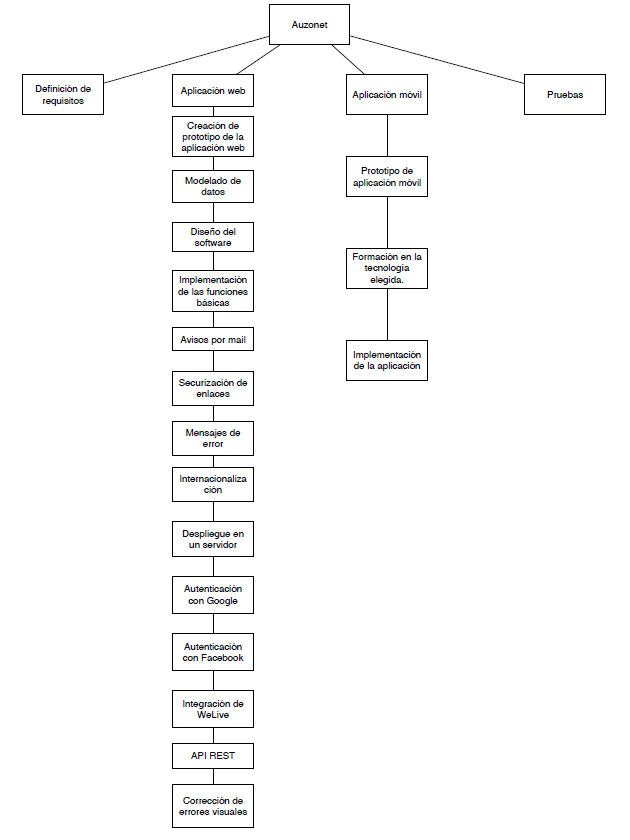
\includegraphics{fig/EDT}
    \caption{EDT}\label{fig:edt}
\end{figure}
\restoregeometry

\section{Organización}
\subsection{Estructura de la organización}
El desarrollo del proyecto se va a llevar a cabo durante la jornada de trabajo en DeustoTech MORELab de 4 horas diarias y solo se contará un un solo recurso humano que hará los siguientes perfiles:

\begin{description}
    \item[Desarrollador de software:] Persona encargada de programar las estructuras de control de la plataforma.
    \item[Diseñador:] Persona encargada de el aspecto final con el que el usuario final va a interactuar.
    \item[Director de proyecto:] Persona a cargo de controlar el progreso del proyecto y de su organización.
    \item[Experto en plataforma WeLive:] Miembro del equipo de MORELab participante del desarrollo de la plataforma WeLive para asesorar técnicamente al equipo.
\end{description}

Cada dos semanas se hará una sesión en la que se valorará el trabajo realizado y los cambios necesarios y si ya constituye suficiente producto como para considerar lo hecho una unidad funcional.

\section{Estimación de cargas de trabajo}
\begin{itemize}
    \item 1. Definición de requisitos: 15
    \item 2. Aplicación web: 171
    \begin{itemize}
        \item 2.1. Creación de prototipo de la aplicación web: 15
        \item 2.2. Modelado de datos: 9
        \item 2.3. Diseño del software: 15
        \item 2.4. Implementación de las funciones básicas del portal: 45
        \item 2.5. Creación de un sistema de usuarios: 18
        \item 2.6. Implementación de los avisos por mail: 9
        \item 2.7. Securización de enlaces: 3
        \item 2.8. Mensajes de error: 3
        \item 2.9. Internacionalización: 6
        \item 2.10. Despliegue en servidor: 12
        \item 2.12. Autenticación con Google: 6
        \item 2.13. Autenticación con Facebook: 6
        \item 2.14. Integración con WeLive: 6
        \item 2.15. API Rest: 12
        \item 2.16. Corrección de errores visuales en pantallas de alta densidad: 3
    \end{itemize}
    \item 3. Aplicación móvil: 60
    \begin{itemize}
        \item 3.1. Prototipo de aplicación móvil: 3
        \item 3.2. Formación en la tecnología elegida para el desarrollo: 12
        \item 3.3. Implementación de la app móvil: 45
    \end{itemize}
    \item 4. Pruebas: 12
\end{itemize}
\section{Reparto de cargas de trabajo}
A continuación, se especifica la carga de trabajo èstimada para cada perfil del proyecto sobre el total de 258:
\begin{description}
    \item[Desarrollador de software:] 218
    \item[Diseñador:] 22
    \item[Director de proyecto:] 15
    \item[Experto en plataforma WeLive:] 3
\end{description}

\section{Diagrama de GANTT}
\begin{figure}[H]
    \centering
    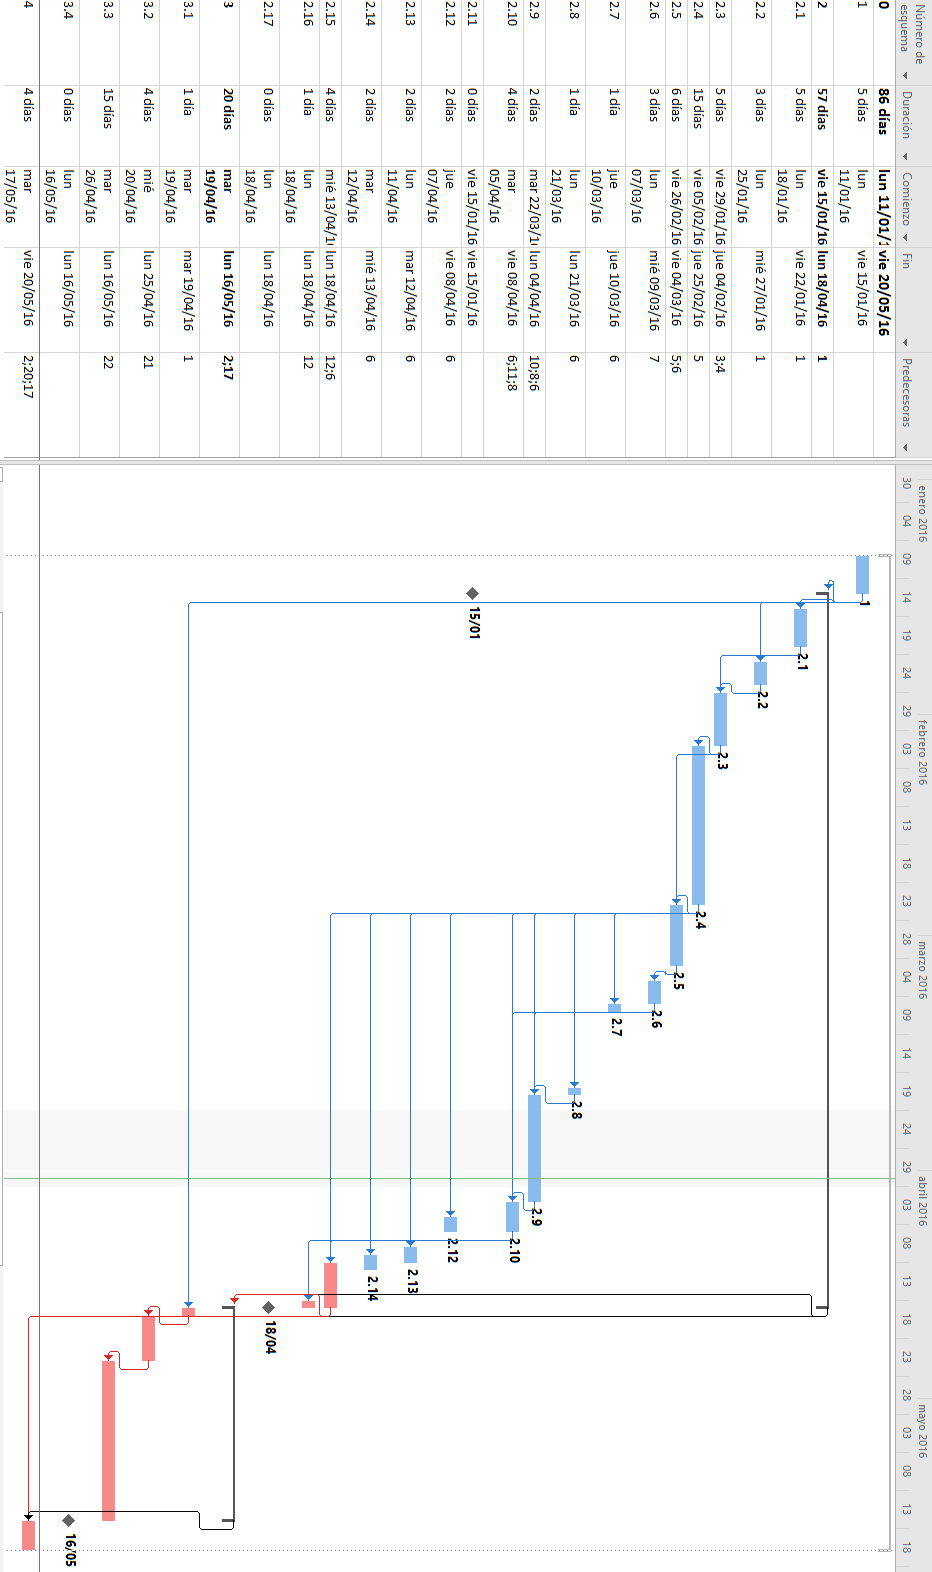
\includegraphics[width=350pt]{fig/gantt}
    \caption{Diagrama de GANTT}\label{fig:gantt}
\end{figure}

\section{Diagrama de precedencia}
\begin{figure}[H]
    \centering
    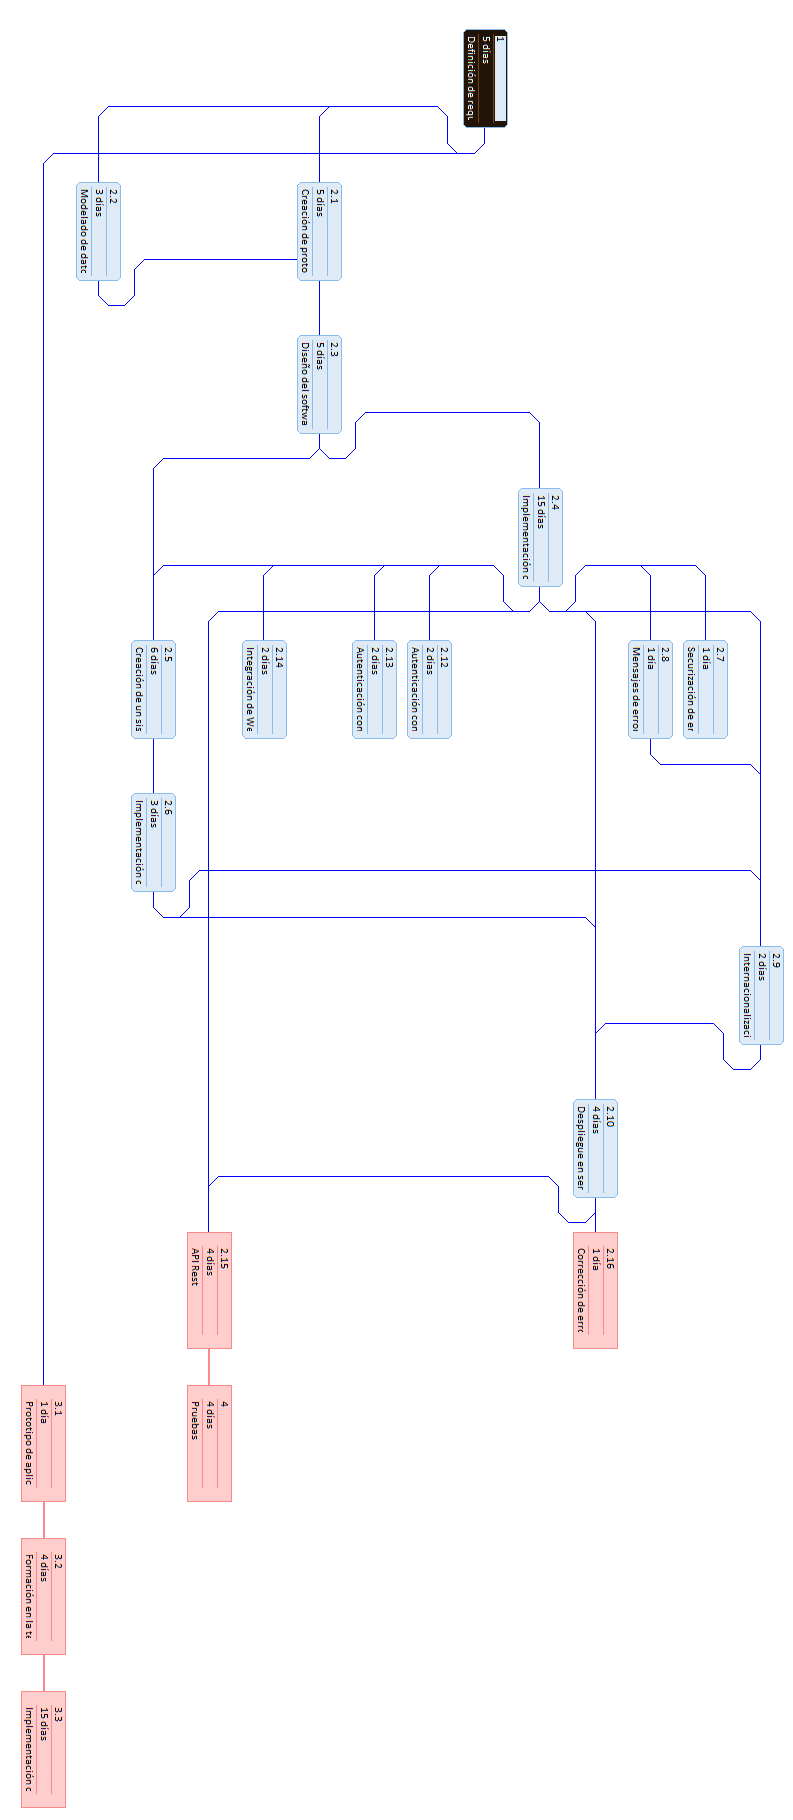
\includegraphics[width=280pt]{fig/precedencia}
    \caption{Diagrama de precedencia}\label{fig:precedencia}
\end{figure}

\section{Presupuesto orientativo}
\begin{table}
  \centering
  \caption{Ejemplo de un entorno tabulado.}\label{tab:ejemplo}
  \begin{tabular}{cccc}
    \toprule
      \textbf{Nombre} & \emph{Valor 1} & \emph{Valor 2} & \emph{Valor 3}\\
    \midrule
      Pedro  & 100     & 200     & 300 \\
      Juan   & 200     & 100     & 600 \\
      Mar\'ia& 300     & 50      & 200 \\
      Carmen & 400     & 10      & 7000\\
    \bottomrule
  \end{tabular}
\end{table}

\printbibliography[heading=bibintoc]

\appendix

\backmatter

\end{document}
